% -------------------------------------------------------------------------------------------------------------
% --- PREAMBLE ------------------------------------------------------------------------------------------------
% -------------------------------------------------------------------------------------------------------------

\documentclass[twoside, a4paper, 12pt]{article}
\usepackage[utf8]{inputenc}
\usepackage{arabtex}
\usepackage[magyar]{babel}
\usepackage{bookman}
\usepackage{thesis-style}
\usepackage{graphicx,wrapfig}
\usepackage{cite}
\usepackage{url}
\usepackage{hyperref}
\usepackage{amssymb,amsmath}
\usepackage{lipsum}% just to generate text for the example
\usepackage{indentfirst}

\newtheorem{definition}{Definíció}

\renewcommand{\listoffigures}{\begingroup
\tocsection
\tocfile{\listfigurename}{lof}
\endgroup}

\renewcommand{\listoftables}{\begingroup
\tocsection
\tocfile{\listtablename}{lot}
\endgroup}


% --- Code listing def -------------------------------------------------------------------

\usepackage{color}
\usepackage{listings}
%\usepackage{courier} %caused problems for me

\lstdefinelanguage{csharp}{
	alsoletter={@=>},
	morekeywords={ abstract, event, new, struct, as, explicit, null, switch, base, extern, object, this, bool, false, operator, throw, break, finally, out, true, byte, fixed, override, try, case, float, params, typeof, catch, for, private, uint, char, foreach, protected, ulong, checked, goto, public, unchecked, class, if, readonly, unsafe, const, implicit, ref, ushort, continue, in, return, using, decimal, int, sbyte, virtual, default, interface, sealed, volatile, delegate, internal, short, void, do, is, sizeof, while, double, lock, stackalloc, else, long, static, enum, namespace, string },
%	sensitive=true,
	morecomment=[l]{//},
	morecomment=[s]{/*}{*/},
	morestring=[b]",
}

\definecolor{red}{rgb}{0.6,0,0} % for strings
\definecolor{blue}{rgb}{0,0,0.6}
\definecolor{green}{rgb}{0,0.8,0}
\definecolor{cyan}{rgb}{0.0,0.6,0.6}

\lstloadlanguages{[Sharp]C}

\lstset{
	language={[Sharp]C},
	basicstyle=\color{black}\ttfamily\scriptsize, 
	tabsize=4, 
	extendedchars=true, 
	breaklines=true, 
	stringstyle=\color{blue}\ttfamily\scriptsize, 
	showspaces=false, 
	showtabs=false, 
	xleftmargin=5pt,
	framexleftmargin=5pt,
	framexrightmargin=2pt,
	framexbottommargin=2pt,
	commentstyle=\color{green}\ttfamily\scriptsize,
	showstringspaces=false, 
	keywordstyle=\color{cyan}\ttfamily\scriptsize,
	morekeywords={ abstract, event, new, struct, as, explicit, null, switch, base, extern, object, this, bool, false, operator, throw, break, finally, out, true, byte, fixed, override, try, case, float, params, typeof, catch, for, private, uint, char, foreach, protected, ulong, checked, goto, public, unchecked, class, if, readonly, unsafe, const, implicit, ref, ushort, continue, in, return, using, decimal, int, sbyte, virtual, default, interface, sealed, volatile, delegate, internal, short, void, do, is, sizeof, while, double, lock, stackalloc, else, long, static, enum, namespace, string },
	sensitive=true,
	morecomment=[l]{//},
	morecomment=[s]{/*}{*/},
	morestring=[b]"
}

%\usepackage{caption}
%\DeclareCaptionFont{white}{\color{white}}
%\DeclareCaptionFormat{listing}{\colorbox{blue}{\parbox{\textwidth}{\hspace{15pt}#1#2#3}}} %changed \colorbox{8} to \colorbox{blue} cause 8 is not a color!
%\captionsetup[lstlisting]{format=listing,labelfont=white,textfont=white, singlelinecheck=false, margin=0pt, font={bf,footnotesize}}

\renewcommand{\lstlistingname}{Kódrészlet}% 
\renewcommand{\lstlistlistingname}{Kódrészletek listája}

% --- Code listing def (END) --------------------------------------------------------------




% Töltsd ki a saját szakdolgozatod adataival
\def\THESISTITLE{Sakk-bot Verseny}
\def\THESISAUTHOR{Virágh Tibor}
\def\THESISDEFENCEYEAR{2018}

\def\DEPARTMENT{Programozáselmélet és Szoftvertechnológiai Tanszék}
\def\SUPERVISOR{dr. Gregorics Tibor}
\def\SUPERVISORPOSITION{Tanszékvezető egyetemi docens}

\lstdefinestyle{sharpc}{language=[Sharp]C, frame=lr, rulecolor=\color{blue!80!black}}
\title{\THESISTITLE}
\author{\THESISAUTHOR}
\date{\THESISDEFENCEYEAR}

\begin{document}
\pagestyle{empty}

\begin{titlepage}

\begin{minipage}{0.40\linewidth}

\includegraphics[scale=0.3]{img/elte-cimer}
\end{minipage}
\begin{minipage}{0.50\linewidth}
\begin{center}
Eötvös Loránd Tudományegyetem \\
Informatikai Kar \\
\DEPARTMENT
\end{center}
\end{minipage}

\hrule
\vfill

\begin{center}
\Huge
\textbf{\THESISTITLE}
\normalsize
\end{center}

\vfill

\begin{minipage}[t]{0.5\linewidth}
\begin{flushleft}
\textbf{\SUPERVISOR} \\
\SUPERVISORPOSITION
\end{flushleft}
\end{minipage}
\begin{minipage}[t]{0.5\linewidth}
\begin{flushright}
\textbf{\THESISAUTHOR} \\
Programtervező Informatikus BSc
\end{flushright}
\end{minipage}

\vfill

\begin{center}
Budapest, \THESISDEFENCEYEAR
\end{center}

\end{titlepage}

\cleardoublepage

%place of the thesis subject registration form
\null
\vspace*{\fill}
\begin{figure}[htbp]
	\centering
	
\includegraphics[width=1.0\textwidth]{img/bots_chess.png}
	\caption{Robotok sakkoznak a Futurama \copyright című sorozat egyik epizódjában.}
	\label{fig:bots_chess}
\end{figure}
\vspace*{\fill}
\null
\cleardoublepage

% table of contents
\tableofcontents
\cleardoublepage


\pagestyle{plain}
\setcounter{page}{1}

\newpage

% -------------------------------------------------------------------------------------------------------------
% --- ÖSSZEFOGLALÁS -------------------------------------------------------------------------------------------
% -------------------------------------------------------------------------------------------------------------

\part{Bevezető}
\section{A dolgozatról}
\subsection{A dolgozat célja}
A dolgozat célja a mesterséges intelligencia kurzuson bemutatott \textbf{„kétszemélyes, teljes információjú, véges és determinisztikus, zéró összegű, játékok”} algoritmusainak bemutatása a gyakorlatban, illetve az érdeklődőbb hallgatók bevonása egy olyan játékba, melyen keresztül elmélyíthetik tudásukat ezen algoritmusokból.

E célból a (normál) sakkot vesszük alapul, mely elég bonyolult ahhoz, hogy látványos eredményeket láthassunk, a legtöbben ismerik a szabályait, illetve egy klasszikus példája a fent nevezett játékok halmazának.

A dolgozat "mellékterméke" egy olyan \textit{API interface}, melyhez kapcsolódva nem csak mesterséges intelligenciát megvalósító programok, hanem "sima", emberi játékosok által is használható kliens is írható, így a téma iránt nem érdeklődők is kipróbálhatják magukat például egy mobilalkalmazás vagy egy asztali Windows / Linux alapú kliens megírásában.

\subsection{A sakk története}
A játék neve a perzsa „shāh” szóból ered, amely uralkodót jelent.\footnote{A "sakk-matt" kifejezés pedig a perzsa „Shāh Māt" kifejezésből származik, amelynek jelentése: "a királyt lerohanták” vagy "védtelen”, "legyőzött”.\cite{ChessMateHu}\cite{ChessMateEn}} Története a legendák világába nyúlik vissza. Egy ismert mese szerint egy brahmin találta ki a sakkot. Jutalmul a rádzsától első hallásra jelentéktelennek tűnő fizetséget kért, mindössze annyi búzaszemet, amennyi a sakktábla kockáira a következő szabály szerint képletesen rátehető: az első kockára egy, a másodikra kettő, a harmadikra négy, vagyis az előzőnek mindig duplája. Hamar kiderült, hogy ennyi búza nem terem a Földön, sőt az emberiség egész történelme alatt nem termelt ennyit.

Az első ismert változata valószínűleg Indiában alakult ki. A maihoz képest egyszerűbb volt, de ugyanakkora táblán és ugyanazokkal a bábukkal játszották, a lépések viszont különböztek. 

Indiából először Perzsiába jutott el. Amikor az arabok elfoglalták Perzsiát, a muszlim világ átvette és ennek következményeként el is terjesztette a játékot Dél-Európában. A sakk mai formáját körülbelül a XV.-ik században érte el.

Keleti terjedése már kissé bizonytalan: először Kínába majd Japánba jutott el és közben sokkal nagyobb változásokon ment keresztül.
\textit{Egy kevésbé elfogadott elmélet szerint eredetileg Kínából származik és terjedt el.}\cite{HistoryOfChessHu}\cite{HistoryOfChessEn}

\subsection{A sakk érdekesebb szabályai}
A sakk szabályait nem részleteznénk, ismertnek tételezzük fel, illetve az interneten könnyen hozzáférhető, mint például a \url{http://www.sakk.hu/help/sakk_szabalyok.html} ~\cite{chessrulessakkhu} oldalon. Néhány fontos dolog azért megjegyzendő, amely kissé megbonyolítja a sakk szabályait.

\textit{Egy volt munkahelyemen dekoráció gyanánt ki volt rakva egy sakktábla bábukkal. Ezt az emberek elkezdték használni: kinyomtattak egy papírt, egyik oldalára azt, hogy "fehér jön" a másik oldalára pedig azt, hogy "fekete jön". Ha valakinek volt kedve és ideje, odamehetett, elgondolkodhatott a lépésen, majd miután lépett, megfordította a papírt és várták, hogy valaki lépjen.}

A kérdés az: a meccs "történetének" ismerete nélkül vajon csak a tábla ismeretével kiszámítható-e az összes lehetséges lépés? Ha valaki odalép ehhez a táblához, meg tudja-e mondani az összes lehetséges lépést? A válasz: \textbf{nem}. Vannak különleges lépések, amelyekhez kell ismerni a parti addigi alakulását is. (Sáncolás, en passant)

\subsection{Egy "gondolkodó gép": a Török}
\begin{wrapfigure}{l}{5cm}
	\caption{Kempelen Farkas - A Török}
	\label{fig:the_turk}
	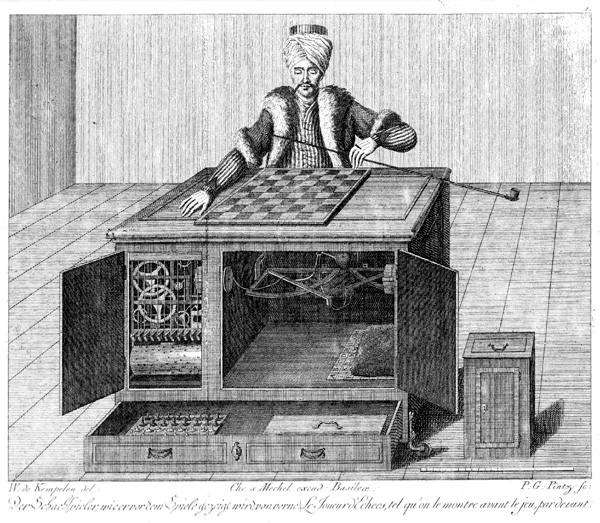
\includegraphics[width=5.0cm]{img/the_turk}
\end{wrapfigure}
A Török Kempelen Farkas álatal 1769-ben alkotott legendás sakkozógép volt, melyet arra épített, hogy elkápráztassa vele Mária Teréziát. A gép sakkpartikat játszott és nyert. Végül végigtúrázta Európát és Észak-Amerikát míg 1854-ben Philadelphiában egy tűzben meg nem semmisült. 

A gép titka nem egy zseniális korát meghaladó "mechanikus mesterséges intelligencia" volt, hanem egy benne elrejtőző emberi kezelő. Ez a gyanú többször is felvetődött, de Kempelen a játszmák előtt felnyitva a gépet mutatta be, hogy nincs senki a gépben. Valójában az eléggé apró termetű kezelő el tudott bújni, amíg elöl illetve hátul is kinyitották a szerkezetet, hogy belenézhessenek. A gépet végül 1857-ben leplezte le nyíltan a The Chess Monthly című amerikai sakklap.\cite{MechanicalTurkHu}\cite{MechanicalTurkEn}

\subsection{Deep Blue}
\begin{wrapfigure}{r}{4cm}
	\caption{Deep Blue}
	\label{fig:deepblue}
	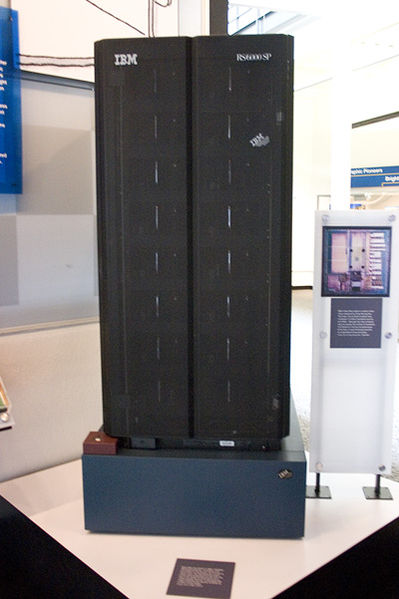
\includegraphics[width=4.0cm]{img/deepblue.jpg}
\end{wrapfigure}
A Deep Blue az IBM által körülbelül 20 millió dolláros költséggel kifejlesztett számítógépe, amely sakkjátékban 1997-ben egy szabályszerű hatjátszmás páros mérkőzésen New Yorkban legyőzte Garri Kaszparovot, az emberi sakkozás akkori világbajnokát.

Első meccs-győzelmét 1996 február 10.-én érte el a világbajnok ellen, de Kasparov három partit nyert és kettőt hozott ki döntetlenre, így 4-2-re győzött a számítógép ellen.

Ezután Deep Blue-t továbbfejlesztették és ekkor már 3,5–2,5-re verte Kasparov-ot 1997 májusában, és ezzel az első számítógépes rendszer lett, amely meg tudta verni az aktuális sakk-világbajnokot a sakkbajnokságokra jellemző időmegszorítás mellett. Kasparov csalást gyanított, és követelt egy visszavágót, ám ebbe az IBM nem ment bele. \cite{DeepBlueHu}\cite{DeepBlueEn}

% -------------------------------------------------------------------------------------------------------------
% --- FEJLESZTŐI DOKUMENTÁCIÓ ---------------------------------------------------------------------------------
% -------------------------------------------------------------------------------------------------------------
\newpage
\part{Fejlesztői Dokumentáció}
\subsection{Bevezető}

A programcsomag három fontos területet fed le, felelősségeik a következők:

\begin{itemize}
	
	\item \textbf{Játék-reprezentáció}
	\begin{itemize}
		\item Definiálja a reprezentációhoz szükséges interface-eket.
		\item Implementálja a sakk reprezentációját és mechanikáját.
		\item Könnyen használható és kiterjeszthető más alkalmazásokban.
	\end{itemize}

	\item \textbf{Algoritmusok}
	\begin{itemize}
		\item Definiál egy interface-t
		\item Tartalmazza néhány algoritmus általános implementációját:
		\begin{itemize}
			\item Minimax
			\item Alfa-béta
			\item Egyéb egyszerűbb példák (random, mohó)
		\end{itemize}
		\item Könnyen használható és kiterjeszthető más alkalmazásokban.
	\end{itemize}

	\item \textbf{Infrastruktúra}
	\begin{itemize}
		
		\item \textbf{Szerver}
		\begin{itemize}
			\item Felhasználó regisztrációja / hitelesítése / nyomonkövetése.
			\item Ellenőrzi a kliensektől jövő lépések érvényességét.
			\item Közvetíti a kliensek felé a partik alakulását.
		\end{itemize}
	
		\item \textbf{Kliens (humán vagy MI kliens)}
		\begin{itemize}
			\item Felhasználó beléptetése, nyomonkövetése.
			\item Közvetíti a felhasználó felé a partik alakulását.
			\item A játékos döntéseit közvetíti a szerver felé.
			\item Példakliensek implementálása:
			\begin{itemize}
				\item Android alkalmazás emberi játékosoknak.
				\item MI bot alkalmazás / alkalmazások melyek különböző algoritmusokat használnak.
			\end{itemize}
		\end{itemize}
	\end{itemize}
\end{itemize}

\newpage
\section{Játék-reprezentáció}
\subsection{Elemzés}
A bevezetőben láthattuk, hogy a következő lehetséges lépések megállapításához nem elég a "táblát látni", kell hozzá még néhány többletinformáció. Ilyen például a már említett bábuk cimkézése illetve ezt helyettesítve (vagy ezzel együtt alkalmazva) a játszma addigi lépéseinek nyilvántartása.

A triviális lépésektől eltekintve problémába merülhet fel, ha például a sáncolást vesszük szemügyre: ahhoz, hogy sáncolhassunk, a benne résztvevő bábuknak nem elég a helyükön lenni, de az is elvárás tőlük, hogy nem is mozoghattak előtte. Azaz például a király vagy a bástya habár (miután elmozdult) visszaléphet az eredeti helyére, ám ekkor már nem lehetséges a sáncolás. Másik ilyen példa a kevésbé ismert "\textit{en passant}" ütés. Ez akkor következik be, amikor az ellenfél az egyik gyalogjával kettőt lép előre pont a mi gyalogunk mellé. Ebben az esetben a következő (és csakis a következő) körben leüthető úgy, mintha nem kettőt, csak egyet lépett volna eredetileg előre. Viszont fontos, hogy ha nem ütjük le, akkor a következő körben ezt már nem tehetjük meg. Ezekben az esetekben adódik az ötlet: rakjunk jelzéseket a bábukra: jelezzük, ha már elmozdultak az eredeti helyükhöz képest vagy például a gyalogot megjelölhetjük, hogy "en passant" üthető. (Ez utóbbi jelzőt viszont a következő körben le is kell venni róla.)

Másik érdekes (és versenyeken alkalmazott) szabály az, hogy ha többször fordul elő ugyanaz az állapot, akkor a játékosok felajánlhatnak döntetlent a másiknak. Ehhez viszont ismerni kell az előző lépéseket, a táblára "simán csak ránézve" ezt a szabályt nem lehet alkalmazni.

Ezekből a példákból látszik, hogy nem elég a tábla aktuális állapotának ismerete, ahhoz kell még extra információ is például a bábukról (elmozdult? en passant üthető?) ami mondjuk egy a bábukra tett jelöléssel megoldható lenne, viszont a legutóbb emlegetett problémára nem megoldás: ahhoz kell az előző lépések listája is.

Megjegyzés: \textit{Ennek egyébként egy érdekes hatása lesz majd az alkalmazott reprezentációra: ha a lehetséges lépések kiszámításához elég lenne "ránézni" a táblára, akkor a játékot reprezentáló gráfunk nem lenne fa, hiszen egy bizonyos állapotba több úton is eljuthatunk. Ha azonban belevesszük egy játékállás reprezentációjához a parti addigi történelmét is, akkor az állások egyediek lesznek és a gráfunk fa-szerű lesz.}

\subsection{Tervezés}
\subsubsection{Egy általános táblás játék reprezentációja}

Egy körökreosztott általános táblás játék a következő elemekből áll:

\begin{itemize}
	\item \textbf{Modell} \\
	A játékállás ábrázolása sokrétű lehet. Tárolni kell a játékosok listáját, az aktuális játékost és a játéknak megfelelő állást: táblán lévő bábuk vagy asztalon levő kártyák.
	
	\item \textbf{Szabályok} (avagy játékmechanika) \\
	A szabályok határozzák meg, hogy milyen helyzetben mik a lehetséges lépések. Az ezt kiszolgáló osztály legyen a játékmester, aki hozzányúlhat a reprezentációhoz, így biztosítva, hogy a játék mindig a szabályoknak megfelelően menjen.
\end{itemize}

A fenti felosztásból adódhat a \ref{fig:boardGameAbstractClassDiagram}. ábrán ismertetett osztálydiagram. A \texttt{GameRepresentation} osztály maga a modell. Teljesen "buta", nincs beleépítve logika, csak tárolja a tábla vagy asztal aktuális állapotát és valamilyen módon lehetőséget biztosít a módosítására. Nem szabad semmilyen játék alapelveit beleépíteni, hiszen például egy sakktáblán is lehet többfajta sakkot játszani, amelyek szabályai különbözőek.

A \texttt{Game} osztály a "játékmester", ő az, aki a szabályok szerint módosítja a reprezentációt. Rajta keresztül kell validálni és végrehajtatni a lépéseket, illetve tőle lehet lekérdezni az aktuális meccs állását illetve egyéb fontosabb tulajdonságait.

\begin{figure}[htbp]
	\centering
	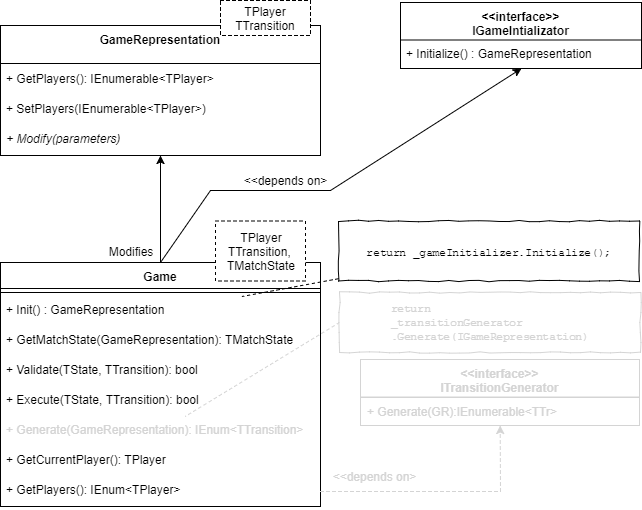
\includegraphics[width=\textwidth]{img/boardGameAbstractClassDiagram.png}
	\caption{Egy általános táblás, körökre osztott játék absztrakt reprezentációja}
	\label{fig:boardGameAbstractClassDiagram}
\end{figure}

A \texttt{Generate()} függvény azért van kiszürkítve az ábrán, mert egy játék lehetséges lépései nem fetétlen diszkrét értékek egy véges halmaza. Szigorúan véve csak azt kell megkövetelni a \texttt{Game} osztálytól, hogy el tudja dönteni egy bejövő lépésről, hogy az érvényes-e. A lépések kigenerálása inkább csak a mesterséges intelligencia algoritmusának "jöhetne jól".

\subsubsection{Sakk reprezentáció}

A sakk is két fő részből áll: reprezentáció és játékmechanika. Ezeket a \texttt{ChessBoard} és a \texttt{ChessGame} osztályok valósítják meg. (Lásd: \ref{fig:chessClassDiagram}. ábra.)

\begin{figure}[htbp]
	\centering
	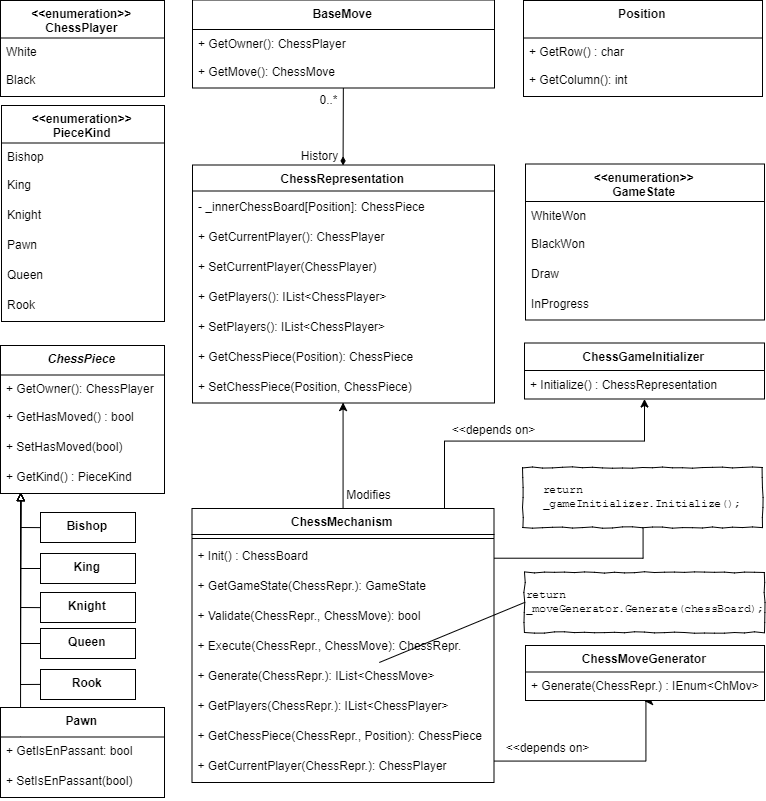
\includegraphics[width=\textwidth]{img/chessClassDiagram.png}
	\caption{Sakkot reprezentáló osztálydiagram}
	\label{fig:chessClassDiagram}
\end{figure}

A \texttt{ChessBoard} osztály önmagában csak reprezentál, minden \textit{property} írható és olvasható. Tartalmazza a játékosok listáját (fehér, fekete), a soronkövetkező játékost, az eddig megtett lépések listáját, illetve a tábla aktuális állapotát az előzőekben már említett jelzőkkel.

A \texttt{ChessGame} osztály felelős a játék kezeléséért, betartja a szabályokat, segít a lehetséges lépések kigenerálásában, validációjában és végrehajtásában. Fontos, hogy a teljes szeparáltság miatt a \texttt{ChessGame} osztálynak kizárólag egy számára átadott \texttt{ChessBoard} osztályból tudnia kell a lehetséges lépéseket, a parti állását, stb.

Felmerülhet, hogy miért nincs egyben ez a két osztály. Ennek több oka van:

\begin{itemize}
	\item \textbf{Egy felelősség alapelve} \textit{(Single responsibility principle)}\cite{SingleResponsibilityHu}~\cite{SingleResponsibilityEn}~\cite{SOLID}~ \\
	Ha egy osztály lenne, az túl bonyolulttá tenné ezt az osztályt: több felelősséget rakna rá és így megsértené a \textit{single responsibility} elvét.
	\item \textbf{Könnyebb felhasználhatóság} \\
	A mesterséges intelligencia algoritmusoknak külön érdekes csak a reprezentáció, hiszen ebből tudnak "állást számolni". Így az aktuális állás osztályozásához nem kell egy mindent tudó objektumot minden egyes lépésben létrehozni, elég csak a reprezentációt átadni a megfelelő kiértékelő függvénynek.
	\item \textbf{Jövőbeli továbbfejleszthetőség} \\
	Sokféle sakkjáték ismeretes, így csak a \texttt{ChessGame} osztály kicserélésével egy másik játékot tudunk készíteni. (Például francia sakk.)
	\item \textbf{Tesztelhetőség} \\
	Ha tiszták és minél egyszerűbbek a különböző részei a játékreprezentációnak, annál könnyebb fókuszált \textit{unit-teszteket} írni ezekre.
\end{itemize}

\subsection{Megvalósítás}

\subsubsection{A sakktábla implementációja}
A sakktáblát reprezentáló \texttt{ChessBoard} osztály az előzőekben részletezett alapelveknek felel meg:
\begin{itemize}
	\item Reprezentálja a táblát.
	\item Nincs szabály beleépítve. \\ 
	(Habár sakkbábukkal és sakklépésekkel dolgozik. Ezt lehetne tovább általánosítani, hogy tényleg csak egy tábla legyen, de a céljainknak egyelőre ez megfelelő.)
\end{itemize}

A legfontosabb függvény a \texttt{Move(from, to)} függvény, amely elvégzi a módosításokat a táblán, ám a \texttt{History}-ba nem írja be, az majd a "játékmester" feladata lesz. Továbbá a \texttt{Move()} függvény visszatérési értéke a "leütött" bábu, vagy \texttt{null} ha üres volt.

\begin{lstlisting}[caption=Sakktábla implementáció vázlat, label=lst:chessboard_code]
public class ChessBoard : IChessBoard, ICloneable<ChessBoard>
{
	private ChessPiece[] pieces = new ChessPiece[64];

	public ChessBoard()	{ /*..*/ }

	public ChessPiece this[Position position]
	{
		get { /* ... */ }
		set { /* ... */ }
	}

	public ChessPlayer CurrentPlayer { get; set; }

	public IEnumerable<ChessPlayer> Players { get; set; }

	public List<ChessMove> History { get; set; }

	public ChessBoard Clone() { /* ... */ }

	public ChessPiece Move(Position from, Position to)
	{
		/* ... */
	}
}
\end{lstlisting}

A sakktáblát egy egydimenziós tömb tárolja, amin a tájékozódás kissé nehézkés, ezért a sakkhoz jobban illő \texttt{Position} tipuson keresztül lesz ez megkönnyítve, amely az algebrai lejegyzést használja:

\begin{lstlisting}[caption=Pozíciók a sakktáblán - Position osztály, label=lst:chessboardposition_code]
/// <summary>
/// Represents a position in the chess board.
/// </summary>
public sealed class Position : IEquatable<Position>
{
	public Position(string notation) { /* ... */ }
	
	public Position(char column, int row) { /* ... */ }
	
	public char Column { get; }
	
	public int Row { get; }
	
	// ...
}
\end{lstlisting}

A későbbi fejlesztések segítéséhez az osztály tartalmaz konvertereket (array index és pozíció között oda-vissza) és egyenlőségvizsgálatot is, hogy írhassuk: \texttt{p1 == p2} vagy \texttt{p1.Equals(p2)}.

\subsubsection{A játékmester implementációja}

A sakk implementációja sokkal bonyolultabb és felvet néhány érdekes problémát. Az implementáló osztály váza a következő:

\begin{lstlisting}[caption=Sakk szabályok implementációja, label=lst:chessgame_code]
public class ChessGame : IMechanism<ChessGameRepresentation, ChessMove, GameState>
{
	public IEnumerable<ChessMove> GenerateMoves(ChessGameRepresentation representation)
	{ 
		/* ... */ 
	}
	
	public GameState GetGameState(ChessGameRepresentation representation)
	{ 
		/* ... */ 
	}
	
	public bool ValidateMove(ChessGameRepresentation representation, ChessMove move)
	{
		return this.GenerateMoves(representation).Contains(move);
	}
	
	public ChessGameRepresentation ApplyMove(ChessGameRepresentation representationParam, ChessMove move)
	{ 
		/* ... */ 
	}
	
	/* ... */
}
\end{lstlisting}

Amint látszik, minden függvény előfeltétele egy reprezentáció. Ebből állapítja meg, hogy mik a lehetséges lépések (\texttt{GenerateMoves}), egy megadott lépés helyes-e az adott helyzetben (\texttt{ValidateMove}) és alkalmazza a megadott lépést ha helyes (\texttt{ApplyMove}).

Ezeket külön-külön megvizsgáljuk:

\paragraph{GenerateMoves()} \mbox{} \\
blah

\paragraph{GetGameState()} \mbox{} \\
blah

\paragraph{ApplyMove()} \mbox{} \\
blah

\subsection{Tesztelés}

asdasdf










\newpage
\section{Algoritmusok}
\subsection{Elemzés}
\subsubsection{A probléma komplexitása}
A sakk reprezentációja tehát már nagyjából látható. Fogalmazzuk meg a problémát: szeretnénk egy olyan programot, amely legyőzi a másik játékost, ami ekvivalens azzal, hogy minden egyes lépésnél a legoptimálisabb lépést választja. Mivel az előzőekben láttuk, hogy ez valószínűleg egy fa bejárása lesz, ezért nem is kell nagyon tovább gondolkodni: megkeressük a fa összes olyan levelét, ahol nyerünk (vagy legalább döntetlent hozunk ki) és megkeressük azt az optimális irányt, amerre haladva ha az ellenfél is a számára legjobb lépést lépi, a nyereségünk maximális lesz.

Tekintsük egy sakkjátszmát: egy átlagos meccs 35-40 fordulós~\cite{averageLengthOfChessGame}\cite{averageLengthOfChessGame2}\cite{chessStatistics}, az átlagos lehetséges lépések száma egy adott állapotból 20\cite{shannonnumber}. Shannon adott egy alsó-korlátot a lehetséges játékok számára, amely $10^{120}$. \footnote{Összehasonlításképp: a világegyetemben levő atomok számát $10^{80}$ darabra teszik, a világegyetem pedig körülbelül $4.32 \times 10^{17}$ másodperce keletkezett, ami kevesebb, mint $10^{18}$-on, ami még így is sok nagyságrenddel kevesebb, mint a lehetséges játékok száma.} Ebből látható, hogy \textit{brute-force} technikával, a jelenlegi technikai háttérrel nem érdemes hozzákezdeni.

Látható, hogy a probléma elég bonyolult és ezért megoldani nem lehet, csak közelíteni. A továbbiakban az algoritmus általánosan fogalmazzuk meg és formalizáljuk, de a sakkon keresztüli példálon mutatjuk be.

\subsubsection{Egy általános táblás játék}
Egy két- (vagy akár több-)személyes, táblás, körökre-osztott játékot meghatározzák a szabályai és a különböző (érvényes) állapotai. A szabályok határozzák meg, hogy mik az érvényes állapotok azáltal, hogy leszűkítik a lehetséges lépéseket olyanokra, amelyek csak érvényes állapotokat eredményeznek.

Ezután már adódik az ötlet: egy játékot reprezentálhatunk egy \textbf{\textit{cimkézett}, irányított gráffal}, ahol a csomópontok a lehetséges állapotok, az élek pedig az átmenetek.

\subsubsection{A probléma, mint útkeresési algoritmus}
Általánosan fogalmazva: a sakk nem más, mint egy körökre osztott két személyes táblás játék. A bevezetőben említett játéktól most kicsit elvonatkoztatva megpróbáljuk megfogalmazni a problémát: egy táblás játék diszkrét lépésekből áll. Kezdetben van egy kezdőállapot, amely meghatározza a lehetséges lépések halmazát, amely lehet egy véges vagy végtelen halmaz. Ezek közül kiválasztva egyet a következő állapotba jutunk, amely megintcsak meghatározza a következő lehetséges lépések halmazát, és így tovább. 

Ezt a legkönnyebben egy \textbf{általános irányított gráfként} képzelhetjük el, ahol a csomópontok a játék lehetséges állapotait tartalmazzák, a köztük levő élek pedig a lépéseket.

Erről a gráfról semmi érdemlegeset nem állíthatunk, nem speciális, hiszen előfordulhat, hogy más utakon is eljuthatunk ugyanazon csúcsba, tehát nagy valószínűség szerint nem fa. Ezt a problémát megszüntethetjük többféle módon, például: 

\begin{itemize}
	\item \textbf{Csomópont duplázással} \\
	Ilyenkor az történik, hogy ha egy állapotba több úton is eljuthatunk, akkor ezeket a csúcsokat többszörözzük. \\
	(Lásd.: \ref{fig:game-graph-transformation} ábra.)
	
	\item \textbf{Ügyes reprezentációval} \\
	Ilyenkor azt tesszük, hogy elgondolkodunk: attól, hogy ugyanabba a csomópontba jutunk több úton, az nem jelenti-e esetleg azt, hogy a más úton elért csúcs már inkább egy másik csúcs. Sakkos példánál maradva: ezt úgy érhetjük el, hogy egy állapot reprezentációjába bevesszük az odavezető utakat. Például előállhat egy hasonló állapot, ha mi is és az ellenfél is előrelép majd vissza ugyanazzal a bábuval.
\end{itemize}

\begin{figure}[htbp]
	\centering
	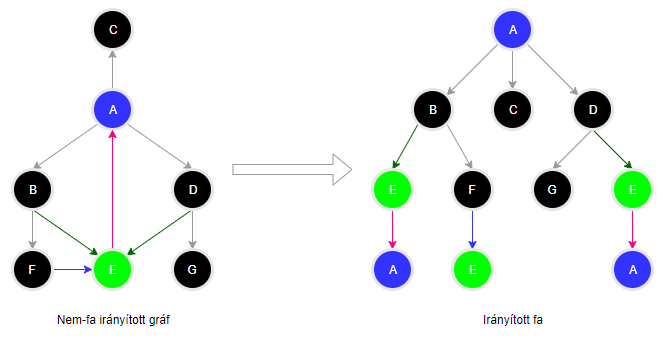
\includegraphics[width=1.0\textwidth]{img/game-graph-transformation.png}
	\caption{Általános irányított gráfból irányított fa konstruálása}
	\label{fig:game-graph-transformation}
\end{figure}

\subsubsection{A Minimax-algoritmus}
\lipsum[1]

\subsubsection{Az alfa-béta algoritmus}
\lipsum[2]

\subsection{Tervezés}
\subsubsection{Általános megfogalmazás}
Az M.I. algoritmusnak "nem kell sokat tudnia": csak annyit várunk el tőle, hogy adjon egy javaslatot a következő lépésre. Természetesen a "hogyan" kérdésre a válasz lehet elég bonyolult is (minimax-, alfa-béta-, genetikus- és tanuló-algoritmusok trükkös heurisztikákkal), de a vége ugyanaz: egy lehetőleg legoptimálisabb lépés kiszámítása.

Ezért az algoritmus interfésze nem is bonyolult: egyetlen függvénye van, a \texttt{TMove Calculate(TState state)}, amely paraméterként kap egy aktuális állapotot (játék-reprezentációt) és visszatér egy lépéssel. (Lásd: \ref{fig:algorithmAbstractDiagram}. ábra.)

\begin{figure}[htbp]
	\centering
	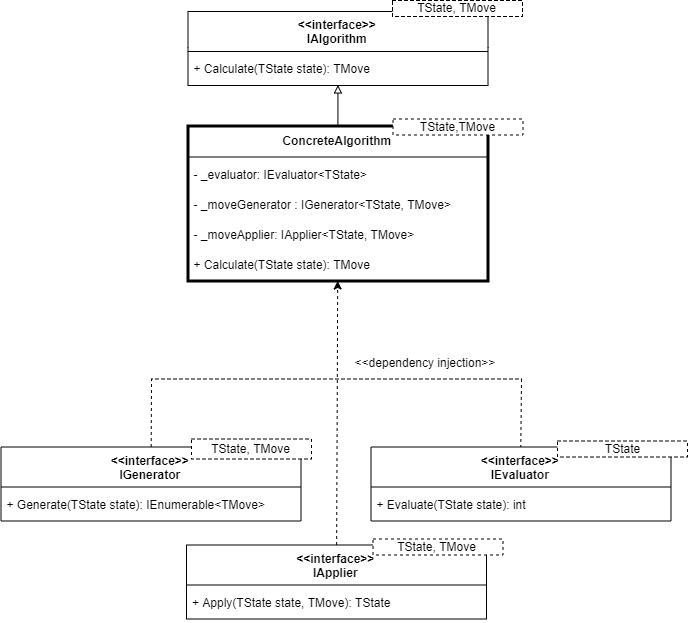
\includegraphics[width=0.7\textwidth]{img/algorithmAbstractDiagram.png}
	\caption{Absztrakt algoritmus interface és függőségei}
	\label{fig:algorithmAbstractDiagram}
\end{figure}

A konkrét megvalósításhoz kellhet egy kis segítség. Az algoritmusnak sok lehetséges lépésből kell kiválasztania a legmegfelelőbbet. Ehhez két dolog kell:

\begin{itemize}
	\item \textbf{Lépés-generátor} \\
	Az algoritmus nem tud semmit a sakkról és nem is kell neki. Azt, hogy milyen lépések lehetségesek, kívülről kell beadni neki. Ez lehet a sakkhoz készült sima generátor osztály, amely egy adott állapotra kigenerálja az összes lehetséges lépést, vagy pedig egy ennek specializált változata, amely egy megfelelő heurisztika alapján csak azokat a lépéseket generálja ki, amelyeket érdemes megvizsgálni, ezzel is csökkentve az algoritmus futási idejét és erőforrásigényét. (Másik felhasználási mód a saját generátorhoz: az is lehetséges, hogy egy játéknak "folytonos" sokaságú lépése létezhet tehát nem kigenerálható, viszont egy bejövő lépésről eldönthető, hogy az érvényes-e. Ez esetben jöhet jól egy olyan generátor-osztály, amely "diszkrét és véges mennyiségű" lehetséges lépést generál.)
	
	\item \textbf{Kiértékelő} \\
	Kell egy kiértékelő-osztály is, amely eldönti az újonnan előállt állapotról annak értékét az aktuális játékos számára. Fontos, hogy a visszaadott érték nem feltétlen kell, hogy egy sima természetes vagy valós szám legyen, de el lehessen dönteni, hogy a visszaadott értékek közül melyik kisebb/nagyobb/egyenlő. Röviden fogalmazva: az \texttt{TResult Evaulate(TState state)} függvénynek a \texttt{TResult} típusának értékeinek halmazának legalább \textbf{részben-rendezett} halmaznak kell lennie.
\end{itemize}

\subsubsection{A Minimax algoritmus}
A Minimax-algoritmus 
Ennek megfelelően implementálható a Minimax algoritmus:

\begin{figure}[htbp]
	\centering
	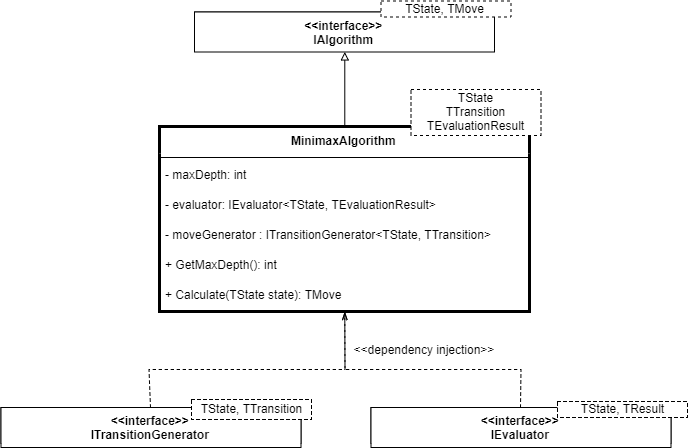
\includegraphics[width=0.7\textwidth]{img/minimaxAbstractDiagram.png}
	\caption{MinimaxAlgorithm osztály}
	\label{fig:minimaxAbstractDiagram}
\end{figure}






\subsection{Megvalósítás}
qwer

\subsection{Tesztelés}

asdasdf


\newpage
\section{Infrastruktúra}
\subsection{Elemzés}
asdf


















\subsubsection{Architektúra}
Az architektúra alapja egy sima szerver-kliens kapcsolat: (\ref{fig:highLevelArchitecture} ábra.)

\begin{figure}[htbp]
	\centering
	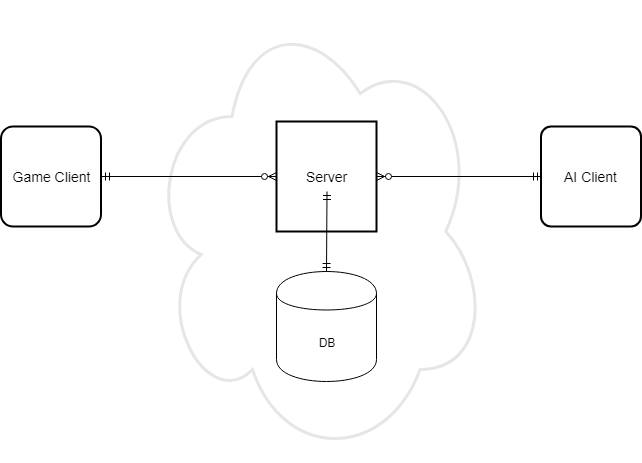
\includegraphics[width=1.0\textwidth]{img/highLevelArchitecture.png}
	\caption{Magas-szintű architektúra}
	\label{fig:highLevelArchitecture}
\end{figure}

A szerver egy \textbf{RESTful} szolgáltatást nyújt a kliensek felé.

\subsubsection{RESTful szolgáltatás}
Néhány szó a REST-ről, hivatkozással...

\subsubsection{Kommunikáció a szerver és a kliensek között}
A kommunikáció \textbf{JSON} üzenetek formájában, HTTP verb-ekkel és HTTP status kódokkal történik, ahogy a \ref{fig:clientServerCommunication} ábrán látható.

\begin{figure}[htbp]
	\centering
	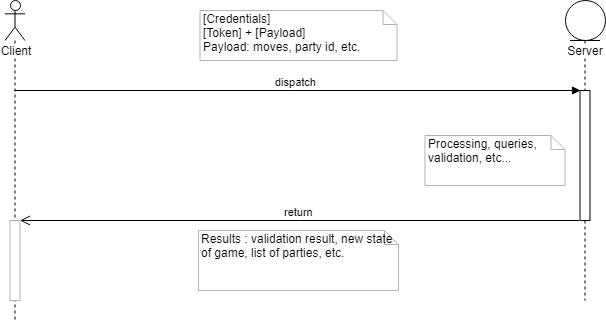
\includegraphics[width=0.8\textwidth]{img/clientServerCommunication.png}
	\caption{Kliens - szerver közötti kommunikáció sémája}
	\label{fig:clientServerCommunication}
\end{figure}


\subsubsection{Szerver}
A szerver feladata a bejövő kérések kiszolgálása. Ő felel a felhasználók beléptetéséért, nyomonkövetéséért és a játékok kezeléséért. A legtöbb funkció kívülről egy nyílt API-n keresztül elérhető, kivétel a felhasználói regisztráció és adminisztráció,
A szerver rendelkezik egy felhasználói felülettel, ahol a regisztráció és felhasználói adatmódosítás elérhető, illetve innen lehet elérni különböző a játékkal kapcsolatos anyagokat is, mint például az API dokumentáció.

\subsubsection{Szerver oldali UI}
Minimalista design, csak az előbb említet funkciókat kiszolgáló UI-t tartalmazza (\ref{fig:serverUiMainScreen}. ábra):

\begin{figure}[htbp]
	\centering
	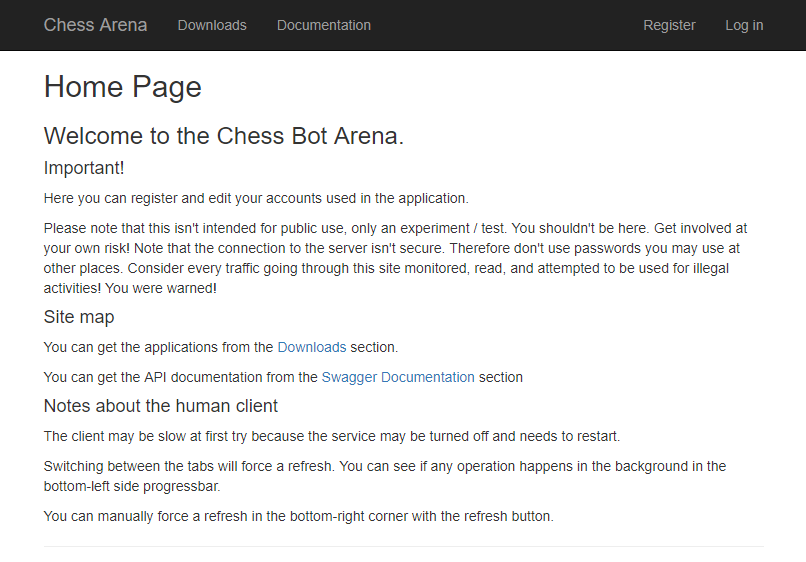
\includegraphics[width=1.0\textwidth]{img/serverUiMainScreen.png}
	\caption{Szerver fő felület}
	\label{fig:serverUiMainScreen}
\end{figure}

A később részletezett open-API dokumentációját a swagger nevű generátorral oldottuk meg, amely felépítését mutatja a \ref{fig:serverUiDocumentation}. ábra.

\begin{figure}[htbp]
	\centering
	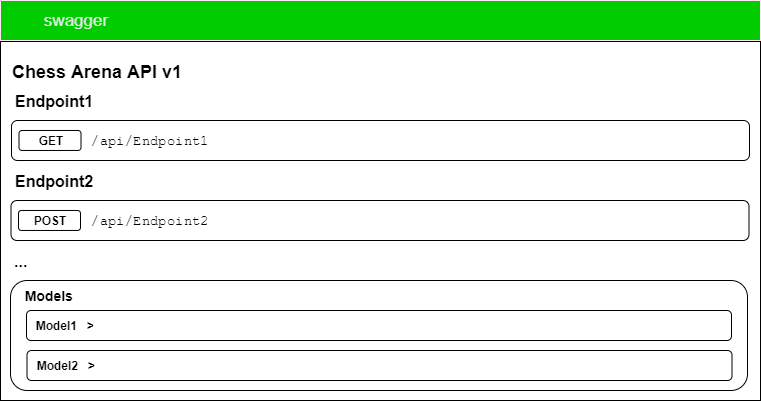
\includegraphics[width=1.0\textwidth]{img/serverUiDocumentation.png}
	\caption{Szerver - generált dokumentáció}
	\label{fig:serverUiDocumentation}
\end{figure}


\subsubsection{Publikus API}
A szerver a következő publikus szolgáltatásokat nyújtja:

% == Szerver - felhasználói fiókok =======================================================================================
\begin{longtable}[c]{|c|p{14cm}|}
\hline
\rowcolor[HTML]{6665CD}
\multicolumn{2}{|l|}{\cellcolor[HTML]{6665CD}{\color[HTML]{FFFFFF} \textbf{Szerver funkciói}}} \\ \hline
\endfirsthead
%
\multicolumn{2}{c}%
{{\bfseries Table \thetable\ folytatása az előző oldalról...}} \\
\hline
\rowcolor[HTML]{6665CD} 
\multicolumn{2}{|l|}{\cellcolor[HTML]{6665CD}{\color[HTML]{FFFFFF} \textbf{Szerver funkciói}}} \\ \hline
\endhead

% -----------------------------------------------------------------------------------------------------------------------
\rowcolor[HTML]{CBCEFB} 
\textbf{1}
&	Bejelentkezés
\\ \nobreakhline

\textbf{GIVEN} &
A szerver fut.
\\ \nobreakhline

\textbf{WHEN} &
Beérkezik egy bejelentkezési kérés egy felhasználói névvel és jelszóval.
\\
\nobreakhline

\textbf{THEN} &
A szerver a felhasználói név és jelszó ellenőrzése után visszajelez a kliensnek.
Ha sikeres volt a belépés, akkor kap egy "token"-t. Más esetben hibajelzést kap.
\\
\hline

% -----------------------------------------------------------------------------------------------------------------------
\rowcolor[HTML]{CBCEFB} 
\textbf{2}
&	Belépési token meghosszabbítása
\\ \nobreakhline

\textbf{GIVEN} &
A szerver fut.
\\ \nobreakhline

\textbf{WHEN} &
Beérkezik egy kérés egy tokennel azzal a szándékkal, hogy az érvényessége meg legyen hosszabbítva.
\\
\nobreakhline

\textbf{THEN} &
A szerver leellenőrzi a token-t és ha még érvényes, akkor egy meghosszabbított token-t ad vissza. Egyébként hibát jelez.
\\
\hline

% -----------------------------------------------------------------------------------------------------------------------
\rowcolor[HTML]{CBCEFB} 
\textbf{3}
&	Szerver-státusz lekérdezése ("Health-check")
\\ \nobreakhline

\textbf{GIVEN} &
-
\\ \nobreakhline

\textbf{WHEN} &
Beérkezik egy kérés a szerverhez, amelyben a kliens érdeklődik a szerver státusza (fut-e?) iránt.
\\
\nobreakhline

\textbf{THEN} &
Ha a szerver fut, akkor visszaküldi a verziószámát. Egyébként nem válaszol.
\\
\hline

% -----------------------------------------------------------------------------------------------------------------------
\rowcolor[HTML]{CBCEFB} 
\textbf{4}
&	Játékosok lekérdezése
\\ \nobreakhline

\textbf{GIVEN} &
A szerver fut, a kliens rendelkezik érvényes token-nel.
\\ \nobreakhline

\textbf{WHEN} &
Beérkezik egy kérés a szerverhez, amelyben a kliens lekéri a játékosok listáját.
\\
\nobreakhline

\textbf{THEN} &
A szerver visszaküldi a játékosok listáját (ha érvényes volt a token).
\\
\hline

% -----------------------------------------------------------------------------------------------------------------------
\rowcolor[HTML]{CBCEFB} 
\textbf{5}
&	Partik lekérdezése
\\ \nobreakhline

\textbf{GIVEN} &
A szerver fut, a kliens rendelkezik érvényes token-nel.
\\ \nobreakhline

\textbf{WHEN} &
Beérkezik egy kérés a szerverhez, amelyben a kliens lekéri az aktuális játékos partijainak listáját.
\\
\nobreakhline

\textbf{THEN} &
A szerver visszaküldi a partik listáját (ha érvényes volt a token).
\\
\hline

% -----------------------------------------------------------------------------------------------------------------------
\rowcolor[HTML]{CBCEFB} 
\textbf{6}
&	Lépés
\\ \nobreakhline

\textbf{GIVEN} &
A szerver fut, a kliens rendelkezik érvényes token-nel.
\\ \nobreakhline

\textbf{WHEN} &
Beérkezik egy kérés a szerverhez, amelyben a kliens közli, hogy melyik partin milyen lépést szeretne kezdeményezni.
\\
\nobreakhline

\textbf{THEN} &
A szerver ellenőrzi, majd végrehajtja és lementi a lépést, erről visszaigazolást küld a legfrisebb állással (ha érvényes volt a token).
\\
\hline

\caption{Szerver alapfunkciói - API}
\label{userStories:server:api}\\
\end{longtable} 

\vbox{
\subsubsection{Dokumentáció}
Az API dokumentációt a \textit{swagger}\cite{swaggerHomepage} generálja a kód, az annotációk és '\textit{summary}' tag-ek alapján.

A swagger generál egy az API-t leíró sémafile-t is, amelyet felhasználva a swagger oldalán generáltathatunk egy kliens a legtöbb nyelvre.

\begin{lstlisting}[caption=Health-check példakód 'summary' tag-ekkel., label=lst:healtcheck]
/// <summary>
/// The health controller. Only used to return the version information.
/// (Can only respond when the service is up and running.)
/// </summary>
[Route("api/Health")]
public class HealthController : Controller
{
    /// <summary>
    /// Health check. Returns the version number of the service.
    /// </summary>
    /// <returns>The version information of the service.</returns>
    [ProducesResponseType(typeof(string), (int)HttpStatusCode.OK)]
    [HttpGet]
    public async Task<IActionResult> Get()
    {
         var version = Microsoft.Extensions
                                .PlatformAbstractions
                                .PlatformServices
                                .Default
                                .Application
                                .ApplicationVersion;

         return Ok(version);
    }
}
\end{lstlisting}

A fenti kódban a \texttt{Get()} függvény \textit{summary} szövege lesz az API végpont dokumentációjában, a \texttt{ProducesResponseType} attribute class-szal pedig jelezhetjük, hogy milyen HTTP státuszjelzés mellett milyen modell jön vissza a szervertől. Például: '200 OK' mellett visszajön egy várt komplex objektum, de mondjuk '500 ERROR' mellett visszajön egy komplex hibaobjektum, nem csak maga a hibakód és az esetleges hibaüzenet.}

\subsubsection{A Kliens}

\subsubsection{Felhasználó és játékos}

Mivel az MI és a játékkliens csak annyiban tér el, hogy ki hozza meg a döntést egy játszmában, ezért a dolgozat további részében fontos lesz a \textbf{„felhasználó”} és a \textbf{„játékos”} megkülönböztetése.

\begin{definition}[Játékos]
Játékos alatt azt értjük, aki "játszik", azaz meghozza a döntéseket. Ez botok esetén a gépi ellenfél, a sima játékkliens esetén az ember lesz.
\end{definition}

\begin{definition}[Felhasználó]
Felhasználó alatt a továbbiakban mindig az emberi \textit{játékost} értjük.
\end{definition}

\subsubsection{Alapfunkciók}
A klienseknek a következő alapfunkcionalitást kell minimum kiszolgálniuk:

% == Kliens - indulás ===================================================================================================
\begin{longtable}[c]{|c|p{14cm}|}
\hline
\rowcolor[HTML]{6665CD}
\multicolumn{2}{|l|}{\cellcolor[HTML]{6665CD}{\color[HTML]{FFFFFF} \textbf{Kliens indítása}}} \\ \hline
\endfirsthead
%
\multicolumn{2}{c}%
{{\bfseries Table \thetable\ folytatása az előző oldalról...}} \\
\hline
\rowcolor[HTML]{6665CD} 
\multicolumn{2}{|l|}{\cellcolor[HTML]{6665CD}{\color[HTML]{FFFFFF} \textbf{Kliens indítása}}} \\ \hline
\endhead
%
\rowcolor[HTML]{CBCEFB} 

% -----------------------------------------------------------------------------------------------------------------------
\textbf{1}
&	Alkalmazás indítása
\\ \nobreakhline

\textbf{GIVEN} &
A kliens telepítve van.
\\ \nobreakhline

\textbf{WHEN} &
A felhasználó jelzi a játék indításának szándékát.
\\
\nobreakhline

\textbf{THEN} &
A kilens elindul és:
\begin{itemize}
	\item Ha a játékos már be van lépve, akkor belép a lobbiba.
	\item Ha a játékos nincs belépve, akkor megjelenik a hitelesítési felület.
\end{itemize} 
\\
\hline

\caption{Kliens alapfunkciói - indítás}
\label{userStories:client:start}\\
\end{longtable} 


% == Kliens - hitelesítési felület ======================================================================================
\begin{longtable}[c]{|c|p{14cm}|}
\hline
\rowcolor[HTML]{6665CD}
\multicolumn{2}{|l|}{\cellcolor[HTML]{6665CD}{\color[HTML]{FFFFFF} \textbf{Kliens - Hitelesítési felület}}} \\ \hline
\endfirsthead
%
\multicolumn{2}{c}%
{{\bfseries \thetable\ folytatása az előző oldalról...}} \\
\hline
\rowcolor[HTML]{6665CD} 
\multicolumn{2}{|l|}{\cellcolor[HTML]{6665CD}{\color[HTML]{FFFFFF} \textbf{Kliens - Hitelesítés}}} \\ \hline
\endhead

% -----------------------------------------------------------------------------------------------------------------------
\rowcolor[HTML]{CBCEFB} 
\textbf{1}
&	Kilépés
\\ \nobreakhline

\textbf{GIVEN} &
Hitelesítési felület aktív.
\\ \nobreakhline

\textbf{WHEN} &
Kilépési szándék jelzése majd annak pozitív megerősítése.
\\
\nobreakhline

\textbf{THEN} &
Alkalmazás bezárása.
\\
\hline

% -----------------------------------------------------------------------------------------------------------------------
\rowcolor[HTML]{CBCEFB} 
\textbf{2}
&	Hitelesítés
\\ \nobreakhline

\textbf{GIVEN} &
Hitelesítési felület aktív.
\\ \nobreakhline

\textbf{WHEN} &
\begin{itemize}
\item Felhasználói név és jelszó megadása.
\item Belépési szándék jelzése.
\end{itemize}
\\
\nobreakhline

\textbf{THEN} &
Adatok elküldése hitelesítésre a szerverhez.
\begin{itemize}
	\item Ha az adatok megfelelőek:
	\begin{itemize}
		\item Felhasználó beléptetése.
		\item Hitelesítési felület elrejtése.
		\item Lobbi megjelenítése, partik állapotának lekérdezése.
	\end{itemize}

	\item Ha az adatok nem megfelelőek:
		\begin{itemize}
			\item Felhasználói tájékoztatása problémáról.
		\end{itemize}
\end{itemize}
\\
\hline

\caption{Kliens alapfunkciói - hitelesítési felület}
\label{userStories:client:authentication}\\
\end{longtable}

% == Kliens - lobbi =====================================================================================================
\begin{longtable}[c]{|c|p{14cm}|}
\hline
\rowcolor[HTML]{6665CD}
\multicolumn{2}{|l|}{\cellcolor[HTML]{6665CD}{\color[HTML]{FFFFFF} \textbf{Kliens - Lobbi}}} \\ \hline
\endfirsthead
%
\multicolumn{2}{c}%
{{\bfseries \thetable\ folytatása az előző oldalról...}} \\
\hline
\rowcolor[HTML]{6665CD} 
\multicolumn{2}{|l|}{\cellcolor[HTML]{6665CD}{\color[HTML]{FFFFFF} \textbf{Kliens - Lobbi}}} \\ \hline
\endhead

% -----------------------------------------------------------------------------------------------------------------------
\rowcolor[HTML]{CBCEFB} 
\textbf{1}
&	Kilépés
\\ \nobreakhline

\textbf{GIVEN} &
A felület aktív.
\\ \nobreakhline

\textbf{WHEN} &
Kilépési szándék, majd annak megerősítése.
\\
\nobreakhline

\textbf{THEN} &
Alkalmazás bezárása.
\\
\hline

% -----------------------------------------------------------------------------------------------------------------------
\rowcolor[HTML]{CBCEFB} 
\textbf{2}
&	Új játék kezdeményezése
\\ \nobreakhline

\textbf{GIVEN} &
A lobbi-felület aktív.
\\ \nobreakhline

\textbf{WHEN} &
Bejelentkezett játékosok közül leendő ellenfél kiválasztva, új játék kezdésének szándéka.
\\
\nobreakhline

\textbf{THEN} &
Új játék kezdeményezésére vonatkozó kérelem elküldése szervernek, majd partik listájának megjelenítése.
\\
\hline

% -----------------------------------------------------------------------------------------------------------------------
\rowcolor[HTML]{CBCEFB} 
\textbf{3}
&	Partik listájának megtekintése
\\ \nobreakhline

\textbf{GIVEN} &
A felület aktív.
\\ \nobreakhline

\textbf{WHEN} &
Partik megtekintésének szándéka.
\\
\nobreakhline

\textbf{THEN} &
Partik felület mutatása.
\\
\hline
\caption{Kliens alapfunkciói - lobbi}
\label{userStories:client:lobby}\\
\end{longtable}

% == Kliens - partik listája ============================================================================================
\begin{longtable}[c]{|c|p{14cm}|}
\hline
\rowcolor[HTML]{6665CD}
\multicolumn{2}{|l|}{\cellcolor[HTML]{6665CD}{\color[HTML]{FFFFFF} \textbf{Kliens - Partik listája}}} \\ \hline
\endfirsthead
%
\multicolumn{2}{c}%
{{\bfseries \thetable\ folytatása az előző oldalról...}} \\
\hline
\rowcolor[HTML]{6665CD} 
\multicolumn{2}{|l|}{\cellcolor[HTML]{6665CD}{\color[HTML]{FFFFFF} \textbf{Kliens - Partik listája}}} \\ \hline
\endhead

% -----------------------------------------------------------------------------------------------------------------------
\rowcolor[HTML]{CBCEFB} 
\textbf{1}
&	Kilépés
\\ \nobreakhline

\textbf{GIVEN} &
A felület aktív.
\\ \nobreakhline

\textbf{WHEN} &
Kilépési szándék, majd annak megerősítése.
\\
\nobreakhline

\textbf{THEN} &
Alkalmazás bezárása.
\\
\hline

% -----------------------------------------------------------------------------------------------------------------------
\rowcolor[HTML]{CBCEFB} 
\textbf{2}
&	Kihívás elfogadása / visszautasítása
\\ \nobreakhline

\textbf{GIVEN} &
A felület aktív, partik listájában egy még nem elfogadott kérés van kiválasztva.
\\ \nobreakhline

\textbf{WHEN} &
Kihívás elfogadása / visszautasítása.
\\
\nobreakhline

\textbf{THEN} &
Kérés elküldése szervernek, partik listájának frissítése.
\\
\hline

% -----------------------------------------------------------------------------------------------------------------------
\rowcolor[HTML]{CBCEFB} 
\textbf{3}
&	Kiválasztott játék megjelenítése
\\ \nobreakhline

\textbf{GIVEN} &
A felület aktív, partik listájában egy már elfogadott játék van kiválasztva.
\\ \nobreakhline

\textbf{WHEN} &
Parti megtekintésének kezdeményezése.
\\
\nobreakhline

\textbf{THEN} &
Játékfelület mutatása.
\\
\hline
\caption{Kliens alapfunkciói - partik listája felület}
\label{userStories:client:parties}\\
\end{longtable}

% == Kliens - játékfelület ==============================================================================================
\begin{longtable}[c]{|c|p{14cm}|}
\hline
\rowcolor[HTML]{6665CD}
\multicolumn{2}{|l|}{\cellcolor[HTML]{6665CD}{\color[HTML]{FFFFFF} \textbf{Kliens - partik listája}}} \\ \hline
\endfirsthead
%
\multicolumn{2}{c}%
{{\bfseries \thetable\ folytatása az előző oldalról...}} \\
\hline
\rowcolor[HTML]{6665CD} 
\multicolumn{2}{|l|}{\cellcolor[HTML]{6665CD}{\color[HTML]{FFFFFF} \textbf{Kliens - partik listája}}} \\ \hline
\endhead

% -----------------------------------------------------------------------------------------------------------------------
\rowcolor[HTML]{CBCEFB} 
\textbf{1}
&	Kilépés
\\ \nobreakhline

\textbf{GIVEN} &
A felület aktív.
\\ \nobreakhline

\textbf{WHEN} &
Kilépési szándék, majd annak megerősítése.
\\
\nobreakhline

\textbf{THEN} &
Alkalmazás bezárása.
\\
\hline

% -----------------------------------------------------------------------------------------------------------------------
\rowcolor[HTML]{CBCEFB} 
\textbf{2}
&	Lépés
\\ \nobreakhline

\textbf{GIVEN} &
A felület aktív.
\\ \nobreakhline

\textbf{WHEN} &
Lépési szándék vagy feladás/döntetlen felajánlása ellenfélnek a sakk szabályai szerint.
\\
\nobreakhline

\textbf{THEN} &
Kérés elküldése szervernek, majd a játékállapot frissítése.
\\
\hline

% -----------------------------------------------------------------------------------------------------------------------
\caption{Kliens alapfunkciói - Játékfelület}
\label{userStories:client:gameScreen}\\
\end{longtable}

A játékkliens képernyői közötti átmenetekért lásd \ref{fig:ClientScreenTransitions} ábra.

\begin{figure}[htbp]
	\centering
	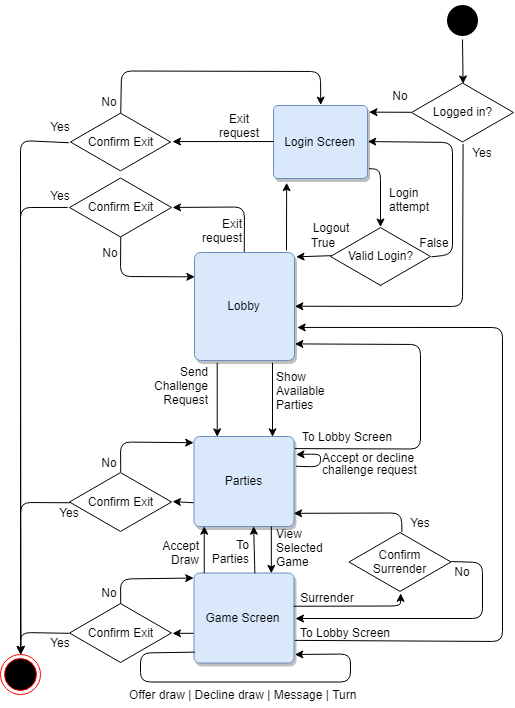
\includegraphics[width=\textwidth]{img/ClientScreenTransitions.png}
	\caption{A játékkliens (telefonos) képernyői közötti átmenetek}
	\label{fig:ClientScreenTransitions}
\end{figure}



\subsubsection{Játékkliens UI terve}
A játékkliens képernyőinek terveit lásd: \ref{fig:gameClientScreens} ábra.
\begin{figure}[htbp]
	\centering
	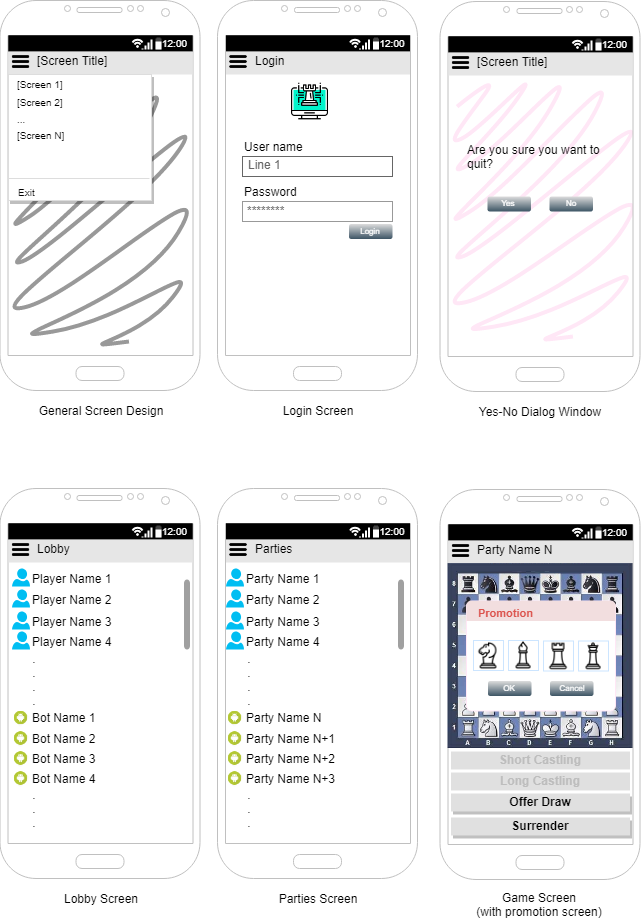
\includegraphics[width=0.8\textwidth]{img/gameClientScreens.png}
	\caption{A játékkliens (telefonos) képernyőinek tervei}
	\label{fig:gameClientScreens}
\end{figure}

\subsection{Tervezés}
asdf

\subsection{Megvalósítás}
qwer

\subsection{Tesztelés}

asdasdf








% -------------------------------------------------------------------------------------------------------------
% --- FEJLESZTŐI DOKUMENTÁCIÓ ---------------------------------------------------------------------------------
% -------------------------------------------------------------------------------------------------------------
\newpage
\part{Felhasználói Dokumentáció}
\subsection{Bevezető}
\lipsum[6-7]
\newpage
\section{Játék-reprezentáció}
\lipsum[1-2]


\newpage
\section{Algoritmusok}
\lipsum[3-4]

\newpage
\section{Infrastruktúra}

\subsection{Szerver}
\lipsum[5-6]

\subsection{Játékkliens}
\lipsum[7-8]

\subsection{MI kliens}
\lipsum[9-10]






\newpage
\bibliographystyle{plain}
\part{\bibname}
\bibliography{szakdolgozat}
%\addcontentsline{toc}{part}{\bibname}
%\printbibliography[heading=none]
%\newpage
\listoffigures
\listoftables
\lstlistoflistings


\end{document}